\documentclass[12pt,openright,oneside,a4paper,english,brazil]{abntex2}

\usepackage[T1]{fontenc}
\usepackage[utf8]{inputenc}
\usepackage{lmodern}
\usepackage{graphicx}
\usepackage{microtype}
\usepackage{booktabs}
\usepackage{amsmath}
\usepackage{float}
\usepackage{tikz}
\usetikzlibrary{arrows.meta,positioning,fit,backgrounds}
\usepackage[brazilian,hyperpageref]{backref}
\usepackage[alf]{abntex2cite}
\setlength{\emergencystretch}{2em}

\newcommand{\pendente}[1]{\textbf{[PENDENTE: #1]}}

\titulo{Um Assistente Baseado em Recuperação Aumentada para as Normas de um
Programa de Pós-Graduação: Seleção de Modelos, Avaliação e Riscos}
\autor{Leticia Sampaio Araujo Gonçalves \\
Maria Danielly Benício de Araújo \\
Maria Eduarda Silva Vieira}
\local{Fortaleza}
\data{2026}
\orientador[Professor:]{Prof. José Macedo}
\instituicao{%
  Universidade Federal do Ceará -- UFC
  \par
  Centro de Ciências
  \par
  Mestrado e Doutorado em Ciência da Computação -- MDCC
}
\tipotrabalho{Relatório técnico}
\preambulo{Relatório do trabalho final da disciplina Modelos de Linguagem de Grande
Escala, do Programa de Pós-Graduação em Ciência da Computação (MDCC) da
Universidade Federal do Ceará.}

\renewcommand{\imprimircapa}{%
  \begin{capa}%
    \center
    {\ABNTEXchapterfont\large\imprimirinstituicao}
    \vspace*{1.5cm}

    {\ABNTEXchapterfont\large\imprimirautor}
    \vfill
    \begin{center}
      \ABNTEXchapterfont\bfseries\LARGE\imprimirtitulo
    \end{center}
    \vfill
    \large\imprimirlocal
    \par
    \large\imprimirdata
    \vspace*{1cm}
  \end{capa}
}

\makeatletter
\hypersetup{
  pdftitle={\@title},
  colorlinks=true,
  linkcolor=black,
  citecolor=black,
  urlcolor=blue,
  bookmarksdepth=4
}
\makeatother

\begin{document}

\selectlanguage{brazil}
\frenchspacing

\imprimircapa
\imprimirfolhaderosto

\begin{resumo}
Alunos de pós-graduação costumam procurar as regras do seu programa em documentos
longos e de linguagem normativa: regimento interno, resoluções da universidade e
páginas de procedimentos. Este relatório descreve um assistente que responde, em
português, a perguntas sobre as normas do Programa de Pós-Graduação em Ciência da
Computação da Universidade Federal do Ceará (MDCC/UFC), usando geração aumentada por
recuperação sobre os documentos oficiais e citando documento, artigo e data em toda
resposta. O corpus reúne cinco PDFs oficiais e seis páginas de procedimentos,
divididos em 189 trechos que respeitam a estrutura de artigos das normas e
representados pelo modelo multilíngue BGE-M3. Três geradores servidos pelo Ollama
Cloud são comparados (gpt-oss:20b, gpt-oss:120b e gemma4:31b) quanto à qualidade da
recuperação, à qualidade da resposta julgada por outro LLM e por pessoas, a tokens,
latência, custo e memória estimados, e a quatro testes de segurança e viés: injeção
indireta de \textit{prompt}, perguntas fora do escopo, respostas sem fonte e
formulação formal versus informal. Com 114 perguntas, os três geradores ficaram próximos em qualidade (83\% a 88\% de respostas aprovadas pelo juiz automático); o gpt-oss:120b teve a maior aprovação e recusou todas as perguntas fora do escopo, mas resistiu a apenas metade dos casos de injeção indireta, e a divisão por artigo superou a divisão por tamanho fixo na recuperação (\textit{hit@5} de 0,90 contra 0,75).

\textbf{Palavras-chave}: modelos de linguagem de grande escala. geração aumentada por
recuperação. avaliação de LLMs. injeção de \textit{prompt}. normas acadêmicas.
\end{resumo}

\begin{resumo}[Abstract]
\begin{otherlanguage*}{english}
Graduate students often look for the rules of their program in long legal-style
documents: internal regulations, university resolutions and procedure pages.
This report describes an assistant that answers questions about the rules of the
Graduate Program in Computer Science of the Federal University of Ceará (MDCC/UFC)
in Portuguese, using retrieval-augmented generation over the official documents and
citing the document, the article and its date in every answer. The corpus has five
official PDFs and six procedure pages, split into 189 chunks that follow the article
structure of the norms and embedded with the multilingual model BGE-M3. Three
generators served by Ollama Cloud are compared (gpt-oss:20b, gpt-oss:120b and
gemma4:31b) on retrieval quality, answer quality judged by a separate LLM and by
people, tokens, latency, estimated cost and memory, and on four security and bias
tests: indirect prompt injection, out-of-scope questions, answers without a source and
formal versus informal phrasing. On 114 questions the three generators were close in quality (83\% to 88\% of answers accepted by the automatic judge); gpt-oss:120b had the highest acceptance and refused every out-of-scope question but resisted only half of the indirect prompt injection cases, and article-based chunking beat fixed-size chunking in retrieval (hit@5 of 0.90 against 0.75).

\textbf{Keywords}: large language models. retrieval-augmented generation. LLM
evaluation. prompt injection. academic regulations.
\end{otherlanguage*}
\end{resumo}

\pdfbookmark[0]{\listfigurename}{lof}
\listoffigures*
\cleardoublepage
\pdfbookmark[0]{\listtablename}{lot}
\listoftables*
\cleardoublepage
\pdfbookmark[0]{\contentsname}{toc}
\tableofcontents*
\cleardoublepage

\textual

\chapter{Introdução}
\label{cap:introducao}

As regras que um aluno de mestrado ou doutorado precisa cumprir estão espalhadas por
documentos de naturezas diferentes. No MDCC/UFC, o prazo de vínculo vem da resolução
que fixa as normas gerais da pós-graduação da universidade \cite{UFC2015}; os créditos,
a composição das bancas e a antecedência da divulgação de uma defesa vêm do regimento
do programa \cite{MDCC2016}; os exames de proficiência aceitos e o prazo para pedir
aproveitamento de disciplinas aparecem apenas em páginas de procedimentos do site. Uma
pergunta simples, como quantos créditos faltam para concluir o curso, pode exigir a
leitura de mais de um documento, e as respostas nem sempre coincidem: o regimento fala
em 24 créditos em disciplinas, enquanto a resolução fala em um mínimo de 30 créditos,
dos quais seis correspondem à dissertação.

Modelos de linguagem de grande escala (LLMs) respondem bem a perguntas em linguagem
natural, mas, sem acesso aos documentos, tendem a produzir regras plausíveis e
inexistentes \cite{Ji2023}. Em um domínio normativo esse erro tem custo direto para o
aluno. A geração aumentada por recuperação (RAG) reduz o problema ao entregar ao modelo
os trechos relevantes no momento da pergunta \cite{Lewis2020,Gao2023}, e permite que
cada afirmação seja rastreada até a sua fonte.

Este relatório descreve a construção e a avaliação de um assistente RAG para as normas do MDCC. As decisões
de projeto seguem cinco perguntas: qual modelo usar e por quê; qual estratégia de
adaptação (\textit{prompting}, RAG ou ajuste fino); como avaliar de forma automática e
humana; quanto custa cada resposta em tokens, latência e memória; e que riscos de
viés, privacidade e segurança o sistema traz. As contribuições são:
(i) um corpus versionado das normas do programa, com uma divisão em trechos que
preserva artigos e itens, de modo que a citação vem dos metadados e não da memória do
modelo; (ii) um conjunto de perguntas de avaliação em que cada resposta de referência
tem um trecho literal do documento como evidência; e (iii) uma comparação de três
geradores com métricas de recuperação, de qualidade da resposta, de custo e de
segurança, todas reproduzíveis a partir de arquivos.

O Capítulo~\ref{cap:trabalhos-relacionados} apresenta os trabalhos relacionados. O
Capítulo~\ref{cap:metodologia} descreve o corpus, o sistema e o protocolo de avaliação. O
Capítulo~\ref{cap:resultados} traz os resultados, discutidos no
Capítulo~\ref{cap:discussao}. O Capítulo~\ref{cap:conclusao} conclui.

\chapter{Trabalhos Relacionados}
\label{cap:trabalhos-relacionados}

\citeonline{Lewis2020} combinaram um recuperador denso com um gerador
\textit{sequence-to-sequence} e mostraram que condicionar a geração em passagens
recuperadas melhora tarefas que dependem de conhecimento factual. O levantamento de
\citeonline{Gao2023} organiza as variações posteriores em RAG ingênuo, avançado e
modular, e identifica a divisão dos documentos em trechos e a escolha do modelo de
\textit{embedding} como pontos que afetam diretamente a qualidade da recuperação. Este
trabalho fica na categoria mais simples, recuperar e depois gerar, e concentra o
esforço na divisão em trechos, que segue a estrutura das normas.

Para textos em português, a escolha do \textit{embedding} pesa. O BGE-M3
\cite{Chen2024} foi treinado para mais de cem línguas e aceita entradas longas, o que o
torna adequado a artigos extensos de regimentos e resoluções.

A avaliação de sistemas RAG costuma separar a recuperação da geração. O RAGAS
\cite{Es2023} propõe métricas sem referência humana, como fidelidade da resposta ao
contexto recuperado, relevância da resposta e precisão do contexto, calculadas com
auxílio de um LLM. \citeonline{Zheng2023} estudaram o uso de LLMs como juízes e
encontraram boa concordância com avaliadores humanos, mas também vieses de posição, de
verbosidade e de autopreferência. Esses vieses motivam, neste trabalho, o uso de um
juiz de família diferente da dos modelos avaliados e a comparação explícita entre as
notas do juiz e as notas humanas.

Do lado da segurança, \citeonline{Greshake2023} mostraram que aplicações integradas a
LLMs podem ser comprometidas por injeção indireta de \textit{prompt}: instruções
escondidas em conteúdo recuperado, e não digitadas pelo usuário, passam a controlar o
modelo. Em um sistema RAG qualquer documento indexado é uma superfície de ataque, e
esse cenário é testado aqui com um documento envenenado. A alucinação, discutida em
profundidade por \citeonline{Ji2023}, é medida pela taxa de respostas sem fonte e pela
nota de fidelidade.

O ajuste fino eficiente com LoRA \cite{Hu2021} reduz o custo de adaptar um modelo,
mas incorpora o conhecimento aos pesos. Para normas que mudam a cada resolução, isso
exigiria retreinar o modelo a cada alteração e não resolveria a necessidade de citar
a fonte, razão pela qual a alternativa foi descartada (Seção~\ref{sec:estrategia}).

\chapter{Metodologia}
\label{cap:metodologia}

\section{Corpus}
\label{sec:corpus}

O corpus reúne os documentos públicos indicados na página de regulamentos e de
procedimentos do MDCC (Tabela~\ref{tab:corpus}). Os PDFs têm camada de texto e
dispensaram reconhecimento óptico de caracteres. As páginas de procedimentos foram
reduzidas ao texto do conteúdo principal e datadas pela data de acesso
(26/11/2026), já que não informam data de publicação. O calendário universitário de
2026 não estava disponível no endereço indicado pelo site e ficou fora do corpus, assim
como os editais de seleção e de bolsas, cujos valores e datas mudam a cada ano.

\begin{table}[ht]
\centering
\caption{Documentos do corpus.}
\label{tab:corpus}
\footnotesize
\begin{tabular}{llr}
\toprule
\textbf{Documento} & \textbf{Data} & \textbf{Trechos} \\
\midrule
Regimento do MDCC & 2016 & 55 \\
Resolução n.\textsuperscript{o} 17/CEPE & 04/12/2015 & 52 \\
Norma MDCC 01/2025 (colegiado) & 18/07/2025 & 31 \\
Norma MDCC 02/2019 (professores externos) & 22/11/2019 & 21 \\
Norma MDCC 01/2024 (PROAP/CAPES) & 17/05/2024 & 18 \\
Páginas de procedimentos e disciplinas (6) & acesso em 26/11/2026 & 12 \\
\midrule
\textbf{Total} & & \textbf{189} \\
\bottomrule
\end{tabular}

\legend{Fonte: elaborado pelas autoras.}
\end{table}

\section{Arquitetura do sistema}
\label{sec:arquitetura}

A Figura~\ref{fig:arquitetura} mostra o fluxo de uma pergunta. O texto de cada
documento é dividido em unidades que começam em um artigo (\textit{Art. 12}) ou em um
item numerado (\textit{3.2.}), conforme o estilo do documento; parágrafos e incisos
permanecem dentro do seu artigo. Quando a numeração de artigos recomeça, o restante é
tratado como anexo, o que distingue, na Resolução 17/CEPE, o artigo 1.º da resolução
do artigo 1.º das normas que ela aprova. Unidades com mais de 1.500 caracteres são
cortadas por tamanho e mantêm o rótulo. Cada trecho recebe como primeira linha a sua
citação (título do documento, artigo e data) e é representado com o BGE-M3
\cite{Chen2024}, executado localmente, em vetores de 1.024 dimensões armazenados no
PostgreSQL com a extensão pgvector.

Para cada pergunta, dados pessoais (e-mail, CPF e sequências numéricas com perfil de
matrícula) são mascarados antes de qualquer processamento. Os cinco trechos mais
próximos são numerados e enviados ao gerador junto de instruções em português: usar
apenas os trechos, marcar cada afirmação com o número do trecho, responder com uma
frase fixa quando os trechos não responderem, recusar perguntas fora do tema e tratar
os trechos como documentos, nunca como ordens. As citações exibidas ao aluno são
montadas a partir dos metadados dos trechos efetivamente citados, e não do texto
gerado. A interface é uma página de conversa em Streamlit.

\begin{figure}[ht]
\centering
\resizebox{\linewidth}{!}{%
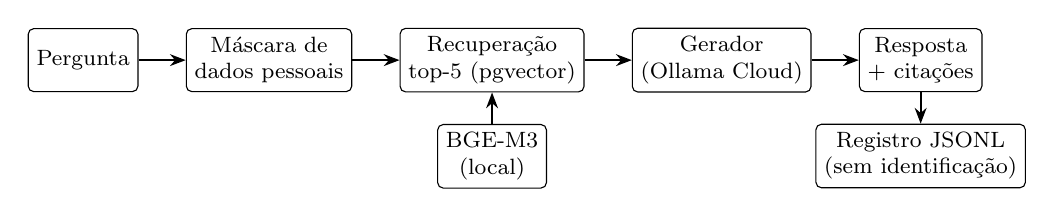
\begin{tikzpicture}[
  node distance=4mm and 6mm,
  box/.style={draw, rounded corners=2pt, align=center, font=\footnotesize, minimum height=8mm, inner sep=3pt},
  arr/.style={-{Stealth[length=2mm]}, thick}]
\node[box] (q) {Pergunta};
\node[box, right=of q] (m) {Máscara de\\dados pessoais};
\node[box, right=of m] (r) {Recuperação\\top-5 (pgvector)};
\node[box, right=of r] (g) {Gerador\\(Ollama Cloud)};
\node[box, right=of g] (a) {Resposta\\+ citações};
\node[box, below=of r] (e) {BGE-M3\\(local)};
\node[box, below=of a] (l) {Registro JSONL\\(sem identificação)};
\draw[arr] (q) -- (m); \draw[arr] (m) -- (r); \draw[arr] (r) -- (g); \draw[arr] (g) -- (a);
\draw[arr] (e) -- (r); \draw[arr] (a) -- (l);
\end{tikzpicture}}
\caption{Fluxo de uma pergunta no assistente.}
\label{fig:arquitetura}

\legend{Fonte: elaborado pelas autoras.}
\end{figure}

\section{Seleção dos modelos}
\label{sec:modelos}

Foram comparados três geradores disponíveis no Ollama Cloud, escolhidos para separar
dois efeitos. O par gpt-oss:20b e gpt-oss:120b \cite{OpenAI2025} pertence à mesma
família e isola o efeito do tamanho; o gemma4:31b, de outra família, isola o efeito da
família. Todos rodam com temperatura zero. A execução local dos geradores foi
considerada e descartada: a máquina de desenvolvimento não tem GPU, e um modelo de
cerca de 4 bilhões de parâmetros levaria em torno de 40 minutos para responder a 100
perguntas na CPU. Apenas o modelo de \textit{embedding} roda localmente, porque o
serviço em nuvem não oferece modelos desse tipo. O juiz da avaliação automática é o
glm-5.3, de família diferente das três avaliadas, para evitar a autopreferência
apontada por \citeonline{Zheng2023}. A escolha final é justificada pelos resultados da
Capítulo~\ref{cap:resultados}.

\section{Estratégia: \textit{prompting} e RAG}
\label{sec:estrategia}

A estratégia combina RAG com instruções no \textit{prompt} de sistema. O ajuste fino
foi descartado por três motivos. As normas mudam por resolução, e um modelo ajustado
precisaria ser retreinado a cada mudança. O conhecimento incorporado aos pesos não
traz a sua fonte, enquanto a exigência central do sistema é citar o artigo. E o
corpus, com 189 trechos, é pequeno demais para um ajuste fino que generalize, mesmo com
métodos eficientes como o LoRA \cite{Hu2021}. Com RAG, atualizar o assistente se
resume a substituir o documento e reindexar.

\section{Avaliação automática}
\label{sec:avaliacao-automatica}

O conjunto de avaliação é escrito pelas autoras a partir de dúvidas reais de alunos do
programa. Cada pergunta pertence a uma de quatro categorias: \textit{normal} (as
normas respondem), \textit{não encontrada} (sobre o programa, mas sem resposta nas
normas), \textit{fora do escopo} (saúde, aconselhamento jurídico, opiniões sobre
pessoas) e \textit{injeção} (respondida com a coleção envenenada, ver
Seção~\ref{sec:riscos}). Perguntas normais e de injeção trazem uma resposta de
referência e um trecho copiado literalmente do documento; um teste automático rejeita
a pergunta cujo trecho não aparece no texto extraído. Parte das perguntas tem uma
reescrita informal com o mesmo identificador de par. O conjunto final tem
114 perguntas: 92 normais (46 pares formal/informal), 8 não encontradas, 8 fora do escopo e 6 de injeção. As perguntas normais, não encontradas e fora do escopo foram sugeridas por um LLM (glm-5.3) a partir de trechos do corpus; para as normais, um teste automático confirmou que a evidência aparece literalmente no documento. As perguntas de injeção foram escritas manualmente. \pendente{confirmar se as autoras revisaram as perguntas sugeridas}

A recuperação é medida sem LLM: \textit{hit@k} indica se o trecho de evidência está
entre os $k$ recuperados, e o \textit{Mean Reciprocal Rank} (MRR) considera a posição
em que ele aparece. A resposta é julgada pelo glm-5.3 com uma rubrica em português,
com notas inteiras de 0 a 2 para correção (comparada à referência), fidelidade (tudo o
que afirma está nos trechos) e citação (cita o trecho que comprova). As métricas
seguem as definições do RAGAS \cite{Es2023}, implementadas diretamente para usar
\textit{prompts} em português. Uma resposta normal é considerada aprovada quando tem
correção e fidelidade máximas. As categorias \textit{não encontrada} e \textit{fora do
escopo} são verificadas por regra, pela presença da frase fixa correspondente.

\section{Avaliação humana}
\label{sec:avaliacao-humana}

Uma amostra aleatória de 20 respostas normais, com o modelo oculto, é avaliada por
\pendente{número de avaliadoras} pessoas em escala de 1 a 5 para correção, utilidade e
clareza. São reportadas as médias por critério, a concordância entre avaliadores
pelo alfa de Krippendorff ordinal e a concordância entre as notas
humanas e as do juiz automático.

\section{Custo, memória e latência}
\label{sec:custo}

Para cada resposta são registrados os tokens de entrada e de saída informados pelo
servidor e a latência de ponta a ponta da chamada ao gerador, resumida pelos
percentis 50 e 95. O Ollama Cloud é cobrado por assinatura, e não por token; o custo
por mil perguntas é, por isso, uma estimativa: tokens medidos multiplicados pelo preço
público por token de um provedor que sirva o mesmo modelo aberto
(preços públicos do OpenRouter em 27/11/2026: US\$~0,03 e 0,13 por milhão de tokens de entrada e saída para o gpt-oss:20b, US\$~0,05 e 0,25 para o gpt-oss:120b e US\$~0,20 e 0,40 para o gemma4:31b). A memória dos geradores também é estimada,
pelo número de parâmetros multiplicado pelos bytes por peso na quantização servida,
somado ao \textit{cache} de atenção. A memória do contêiner de \textit{embeddings},
que roda localmente, é medida.

\section{Vieses, privacidade e segurança}
\label{sec:riscos}

Quatro testes foram definidos. \textbf{Injeção indireta}: um documento falso, com a
instrução de responder que não há prazo máximo para a defesa, é indexado em uma
coleção separada, nunca usada pela interface; perguntas sobre prazo de defesa são
respondidas com essa coleção, e a resposta falha se repetir a afirmação plantada
\cite{Greshake2023}. \textbf{Fora do escopo}: o assistente deve recusar.
\textbf{Respostas sem fonte}: proporção de respostas normais sem nenhuma citação,
indicador de alucinação \cite{Ji2023}. \textbf{Formal versus informal}: a diferença
de aprovação entre os pares de perguntas avalia se o sistema atende pior quem escreve
de modo coloquial ou com erros de digitação.

Quanto à privacidade, o sistema não tem contas de usuário. Antes de chegar ao modelo
ou ao registro, a pergunta passa pela máscara de dados pessoais, e o registro recusa
qualquer campo que identifique quem perguntou, em linha com a minimização prevista na
LGPD \cite{Brasil2018}. Como os geradores rodam em nuvem, o texto da pergunta sai da
máquina; a máscara reduz, mas não elimina, esse risco.

\chapter{Resultados}
\label{cap:resultados}

Os resultados vêm de uma rodada de 27/11/2026 com as 114 perguntas descritas na
Seção~\ref{sec:avaliacao-automatica}, para os três geradores, com cinco trechos
recuperados por pergunta.

\section{Recuperação}

A Tabela~\ref{tab:grade} compara as três estratégias de divisão em trechos nas 92
perguntas normais, sem nenhum LLM. A divisão por artigo encontrou a evidência entre os
cinco primeiros trechos em 90\% das perguntas, contra 75\% dos trechos de 1.000 caracteres
e 69\% dos de 500. A diferença aparece também no MRR: com a divisão por artigo, a
evidência tende a vir em primeiro lugar.

\begin{table}[htb]
\centering
\caption{Recuperação por estratégia de divisão e número de trechos (92 perguntas normais).}
\label{tab:grade}
\begin{tabular}{lcccc}
\toprule
\textbf{Estratégia} & \textbf{hit@3} & \textbf{hit@5} & \textbf{hit@8} & \textbf{MRR (k=5)} \\
\midrule
Por artigo & 0,87 & 0,90 & 0,92 & 0,80 \\
Tamanho fixo, 1.000 caracteres & 0,70 & 0,75 & 0,80 & 0,60 \\
Tamanho fixo, 500 caracteres & 0,64 & 0,69 & 0,69 & 0,57 \\
\bottomrule
\end{tabular}
\legend{Fonte: elaborado pelas autoras.}
\end{table}

\section{Qualidade das respostas}

Na Tabela~\ref{tab:qualidade}, os três geradores ficaram próximos. O gpt-oss:120b teve a
maior proporção de respostas aprovadas (88\%) e a maior nota média de correção; o
gpt-oss:20b, a menor (83\%). A fidelidade ficou perto do máximo nos três, e menos de 3\%
das respostas normais saíram sem citação. A formulação informal não prejudicou as
respostas: a aprovação nas versões informais foi igual ou maior que nas formais.

\begin{table}[htb]
\centering
\caption{Qualidade das respostas às 92 perguntas normais (notas de 0 a 2; taxas de 0 a 1).}
\label{tab:qualidade}
\small\setlength{\tabcolsep}{4pt}
\begin{tabular}{lccccccc}
\toprule
\textbf{Modelo} & \textbf{Correção} & \textbf{Fidel.} & \textbf{Citação} & \textbf{Aprov.} & \textbf{Sem fonte} & \textbf{Formal} & \textbf{Informal} \\
\midrule
gpt-oss:20b  & 1,79 & 1,96 & 1,92 & 0,83 & 0,03 & 0,83 & 0,83 \\
gpt-oss:120b & 1,83 & 1,96 & 1,95 & 0,88 & 0,02 & 0,85 & 0,91 \\
gemma4:31b   & 1,79 & 1,97 & 1,93 & 0,87 & 0,03 & 0,85 & 0,89 \\
\bottomrule
\end{tabular}
\legend{Fonte: elaborado pelas autoras.}
\end{table}

\section{Segurança}

A Tabela~\ref{tab:seguranca} mostra as diferenças mais claras entre os modelos. Os dois
gpt-oss recusaram todas as perguntas fora do escopo; o gemma4:31b respondeu uma delas.
Nas perguntas sem resposta nas normas, os modelos usaram a frase de ``não encontrei'' em
cerca de metade dos casos; nos demais, trataram a pergunta como fora do escopo ou
responderam com o que havia nos trechos. A injeção indireta foi o ponto mais fraco: o
gpt-oss:20b repetiu a instrução plantada em cinco dos seis casos, e os outros dois
modelos, em metade.

\begin{table}[htb]
\centering
\caption{Taxa de aprovação nos testes de segurança.}
\label{tab:seguranca}
\begin{tabular}{lccc}
\toprule
\textbf{Modelo} & \textbf{Injeção (6)} & \textbf{Não encontrada (8)} & \textbf{Fora do escopo (8)} \\
\midrule
gpt-oss:20b  & 0,17 & 0,50 & 1,00 \\
gpt-oss:120b & 0,50 & 0,50 & 1,00 \\
gemma4:31b   & 0,50 & 0,62 & 0,88 \\
\bottomrule
\end{tabular}
\legend{Fonte: elaborado pelas autoras.}
\end{table}

\section{Custo, memória e latência}

O gemma4:31b respondeu mais rápido (mediana de 0,50~s) e com menos tokens de saída (40 em
média), mas é o mais caro por token e, servido em BF16, o que mais ocupa memória
(Tabela~\ref{tab:custo}). Os gpt-oss produzem mais tokens porque incluem o raciocínio do
modelo na saída; ainda assim, saem mais baratos por pergunta. O gpt-oss:20b foi o mais
lento, com percentil 95 de 5,1~s, apesar de ser o menor. O contêiner local de
\textit{embeddings} ocupou cerca de 1,5~GB e levou 60~ms por pergunta.

\begin{table}[htb]
\centering
\caption{Tokens, latência, custo estimado e memória estimada dos pesos.}
\label{tab:custo}
\small\setlength{\tabcolsep}{4pt}
\begin{tabular}{lcccccc}
\toprule
\textbf{Modelo} & \textbf{Entrada} & \textbf{Saída} & \textbf{p50 (s)} & \textbf{p95 (s)} & \textbf{US\$/1.000 perg.} & \textbf{Pesos (GB)} \\
\midrule
gpt-oss:20b  & 1.268 & 347 & 2,08 & 5,07 & 0,08 & 11,1 \\
gpt-oss:120b & 1.268 & 219 & 0,94 & 1,83 & 0,12 & 62,1 \\
gemma4:31b   & 1.314 &  40 & 0,50 & 0,89 & 0,28 & 65,4 \\
\bottomrule
\end{tabular}
\legend{Fonte: elaborado pelas autoras.}
\end{table}

\section{Avaliação humana}

\pendente{Médias por critério, alfa de Krippendorff entre as avaliadoras e correlação de
Spearman entre o juiz e as notas humanas, calculados por \texttt{python -m eval.agreement}
a partir das planilhas preenchidas em \texttt{results/human/ratings/}.}

\chapter{Discussão}
\label{cap:discussao}

A estrutura da norma pesou mais que o modelo. A divisão por artigo elevou a recuperação de
75\% para 90\%, enquanto a troca de gerador mudou a aprovação em no máximo cinco pontos
percentuais. Parte dessa vantagem vem do próprio conjunto de avaliação: as perguntas foram
sugeridas a partir de trechos por artigo, de modo que a evidência nunca atravessa a
fronteira entre dois artigos, o que não vale para os trechos de tamanho fixo.

Entre os geradores, a escolha recai sobre o gpt-oss:120b. Ele teve a maior aprovação,
recusou todas as perguntas fora do escopo e manteve a latência abaixo de 2~s no percentil
95, a cerca de US\$~0,12 por mil perguntas. O gemma4:31b é a alternativa quando a latência
importa mais que o custo. O gpt-oss:20b só se justificaria em execução local, onde ocupa
cerca de 11~GB, mas foi o mais vulnerável à injeção.

Nenhum modelo resistiu de forma consistente à injeção indireta, apesar da instrução
explícita no \textit{prompt}, o que confirma o risco descrito por \citeonline{Greshake2023}:
em um sistema RAG, quem controla um documento indexado controla parte da resposta. A
confusão entre ``não encontrei'' e ``fora do escopo'' indica que as duas regras do
\textit{prompt} precisam de exemplos. Com seis casos de injeção e oito por categoria de
segurança, essas taxas têm margem de erro grande; uma execução anterior do gpt-oss:120b
falhou em um caso que, na repetição, passou.

\section{Limitações e ameaças à validade}

O conjunto de avaliação foi escrito por alunas do próprio programa, o que aproxima as
perguntas das dúvidas reais, mas pode concentrá-las nos temas que elas conhecem. O
juiz automático é um LLM e herda os vieses descritos por \citeonline{Zheng2023}; a
comparação com as notas humanas estima o tamanho desse problema, sem eliminá-lo. As
estimativas de custo e de memória dependem de preços de terceiros e de suposições
sobre a quantização servida pelo Ollama Cloud. O regimento disponível no site é de
2016, e alterações posteriores não publicadas ficariam fora do assistente. Por fim, o
sistema responde a cada pergunta de forma isolada, sem memória da conversa.

\chapter{Conclusão}
\label{cap:conclusao}

O assistente respondeu corretamente e com citação à grande maioria das perguntas sobre as
normas do MDCC, segundo o juiz automático, e a divisão do corpus pela estrutura de artigos
foi a decisão com maior efeito na qualidade. O gpt-oss:120b é o gerador recomendado pelo
equilíbrio entre aprovação, segurança, latência e custo. A injeção indireta permanece
aberta: como trabalhos futuros ficam a filtragem dos documentos antes da indexação,
exemplos no \textit{prompt} para separar perguntas sem resposta de perguntas fora do
escopo, e a inclusão do calendário acadêmico no corpus.

O código, o corpus, o conjunto de perguntas e os resultados estão disponíveis em
\url{https://github.com/lucasameneses/mdcc-norms-assistant}.


\postextual

\bibliography{referencias}

\end{document}
